\documentclass[12pt, a4paper]{article}
\usepackage[utf8]{inputenc}
\usepackage{amsmath}
\usepackage{amsfonts}
\usepackage{amssymb}
\usepackage[hidelinks]{hyperref}
\usepackage[margin=0.75in]{geometry}
\usepackage{graphicx}
\usepackage{subcaption}
\graphicspath{{Images/}}


\setlength\parindent{0pt}
\setlength{\parskip}{1em}

\title{Team 24 Report}
\author{Yuxin Ma \and Derek Chang \and Tianyi Xiong }
\date{March 2021}

\begin{document}

\maketitle

\section{Topic Questions}
In sports betting, an underdog is a team expected to lose a given match. As opposed to betting on winners with low odds/returns, requiring larger wagers and initial capital, betting on underdogs yield outsize returns with smaller wagers. This could be a possible focused strategy when initial capital is limited but there is a steady inflow of funds, especially when combined with other broad betting strategies. 

In the view of this, our team set out to answer:
\begin{itemize}
    \item  Under what conditions (e.g. when/who) are underdogs likely to win, defying bookmakers’ odds? 
    \item By analyzing attributes of outlier winners can we predict when it is favorable to bet against bookmakers?
\end{itemize}


\section{Executive Summary}
We first define a clear underdog: When the odds set by bookmakers against the team is at least 3.5. This is a good number for investigation purposes as it implies a probability of 1/3.5=29$\%$ of the underdog winning, which is less than 33$\%$ of equal odds of Home, Draw and Away.

We explored match data finding outcomes and highest odds for each match. From analysis of odds we observe trends in matches like higher Away odds and less than favourable Draw odds, leading us to decide on dropping the Draw odds to achieve maximum returns.

We aggregated the performances of all underdogs and realised that underdogs actually win 18$\%$ of their matches, being 1.25 times of the mean probability of bookmakers' implied odds of 14$\%$, it points to feasibility of underdog betting. For performances of each underdog, by simulating bets of \$1 on every underdog match, obtaining an insight that 242/322 and 155/322 teams yield profitable returns as Home and Away underdogs respectively. Shockingly, simply betting on every match of the best performing underdog, the returns are 6.3 times the bet amount.

We assigned a ``dogscore" to each team, indicating the profitability of betting on such team. Armed with the scores, we are able to analyse the common attributes of profitable underdogs using exploratory data analysis and linear regression. We found that profitable underdogs are likely to have lower ``buildup play speed", higher ``chance creation crossing" and ``defence pressure", and fitted a linear regression model to the ``dogscore" against various team attributes.

\section{Exploring Match Data}
To begin investigation on the feasibility of betting on underdogs, we explored the match data. 
\subsection{Basic Match Information and Odds}
We first assigned the outcome (1=Homewin, 0=Draw, -1=Awaywin) and the goal difference for each match. From a betting perspective, we always seek for the highest odds to maximise winnings, so we transformed the odds provided by the bookmakers and obtained the maximum for each match’s Home/Draw/Away odds and dropped the matches with no odds provided. 

Inspecting the transformed match data, we observe that overall, the outcome skewed to winning at home being more common (mean outcome=0.17). Comparing Home to Away odds, the odds for betting on Away tend to be much higher.

\begin{table}[!ht]
    \centering
    \begin{tabular}{|c|c|c|}
    \hline & Home Odds & Away Odds \\
    \hline Mean & 2.8 & 5.1 \\
    \hline Max & 36 & 67 \\
    \hline

    \end{tabular}
    \caption{Statistics of Odds}
    \label{tab:my_label}
\end{table}

We also observe that Draw odds scale with underdogs’ odds but for matches resulting in Draw and Draw odds being the highest of the three odds, the max Draw odds caps out at merely 4.26. Due to the lack of robust winnings and for simplification, we drop the data on Draw odds to focus on underdogs’ odds. 

\subsection{Aggregate Underdog Performance}
Next, we filtered the matches for those resulting in an underdog/surprise win.

Inspecting the underdog wins, we observe that underdogs win made up  2913/22597=13$\%$ of all matches (regardless of a clear underdog). 
When only matches with a clear underdog are used, underdog wins increase to 2913/16306=18$\%$. In other words, as a whole, underdogs have an implied odds of 1/0.18=5.56. 

The mean odds provided by bookmakers is 6.96, which is 25$\%$ higher than the implied odds of the underdog wins, so underdog betting seems to have strong promise for positive returns. However, we note that this is the aggregate of all matches, not from perspective of individual matches, indicating the need for further analysis.

\subsection{Individual Underdog Performance}
Before analysing each team, we attempted two separate methods of identifying teams. At first, we simply used the team ID for each match but we upon further inspection, we found that team attributes changed significantly for different years, making them effectively different teams, which was exactly how we treated them (details in Section 5.2). However, the downside is the sample size of matches for each team is several times less than before.

The exploration of individual underdogs is a direct one. We simulate bets of \$1 on every single underdog and obtain each team’s underdog performance. 

We grouped the matches by the underdog team, and for each underdog, we calculated the number of wins and matches played, the bet returns and the underdog performance, which is indicated with a “dogscore”.
$$\text{``Dogscore"} = \frac{\text{Bet Returns}}{\text{Bet Amount}}$$

This accounts for the fraction of wins by each underdog, weighted by the odds provided for each match. We filtered for underdogs that played at least 3 games at home and away each, to prevent low volume outliers from skewing the scores.

Using this dogscore, we are now able to analyse any possible factors of each team resulting in profitable underdog betting. Note that Home and Away are distinct scenarios with their own scores. Upon inspection of dogscores,

\begin{table}[!ht]
    \centering
    \begin{tabular}{|c|c|c|}
    \hline & Home Dogscore & Away Dogscore \\
    \hline Mean & 1.64 & 1.08 \\
    \hline Max & 6.30 & 4.25 \\
    \hline

    \end{tabular}
    \caption{Mean and Max of Dogscores of underdogs}
    \label{tab:my_label}
\end{table}

All teams have, on average, profitable returns ($>1$ times of cost), 242/322 and 155/322 teams yield profitable returns as Home and Away underdogs respectively and perhaps the most surprising insight is that it is possible to yield 6.3 times the bet amount when betting on the best underdog. Table 3 shows examples of overperforming underdogs.

\begin{table}[!ht]
    \centering
    \begin{tabular}{|c|c|c|c|c|}
    \hline & Team & Wins & Matches played & Dogscore \\
    \hline Home & 2012 VVV-Venlo & 5 & 8 & 3.57 \\
    \hline Away & 2009 AJ Auxerre & 7 & 15 & 3.17 \\
    \hline

    \end{tabular}
    \caption{Notable Good Dogs (those with higher sample size)}
    \label{tab:my_label}
\end{table}

Another perspective of underdog betting is to look at favourites’ and their surprise losses. We repeated the above procedure but simulated bets against the favourites to identify underperformers. Where now a “favscore” is assigned which is also the returns divided by cost, where a higher favscore indicates an underperforming favourite. Table 4 shows examples of overperforming underdogs.

\begin{table}[!ht]
    \centering
    \begin{tabular}{|c|c|c|c|c|}
    \hline & Team & Wins & Matches played & Dogscore \\
    \hline Home & 2012 KAA Gent & 6 & 14 & 2.74 \\
    \hline Away & 2014 Borussia Dortmund & 7 & 15 & 2.82 \\
    \hline

    \end{tabular}
    \caption{Notable Bad Favs (those with higher sample size)}
    \label{tab:my_label}
\end{table}

If we can analyse the common attributes of good underdogs and bad favourites, we may be able to pick underdog bets with a good success rate. The numbers provide an idea of good feasibility of betting on underdogs or against favourites but the sample size for each year-based team is too low for statistical significance. We proceed to broaden the analysis by linking results to match conditions and team attributes (which are not discrete like team identity) to find what results in more surprise/underdog wins. 

\section{Exploring Match Conditions}
By intuition, the league, stage (arena), football season and dates (period of the football season) could be predictive factors on the match results.

To explore the possibility, we grouped all matches by the above conditions individually and assigned a ``condition score".
$$\text{``Condition Score"} = \frac{\text{Underdog Wins with specified condition}}{\text{Matches Played with specified condition}}$$
The dates were transformed into weeks, since matches were usually played weekly, to check if the week segment of a season affects the underdog wins. Plotting the scores for each condition, with a mean reference line, we can find outlier conditions resulting in more underdog wins.

\begin{figure}[!ht]
    \centering
    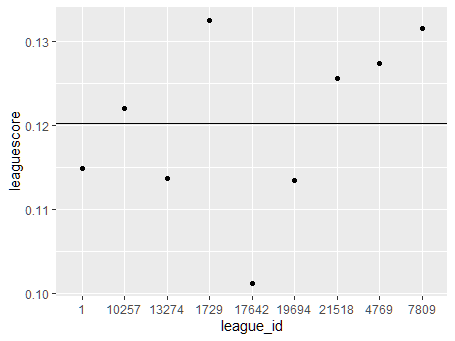
\includegraphics{league.png}
    \caption{leaguescore}
    \label{fig:league}
\end{figure}
Italy Serie A, England Premier League, Spain LIGA BBVA, France Ligue 1 and Germany Bundesliga have above average proportions of underdog wins. They happen to be the top leagues in terms of popularity and competition. This may indicate that at the highest levels of football, the underdogs are more unpredictable as there may be a saturation of differentiation in top skill level. 

\begin{figure}[!ht]
    \centering
    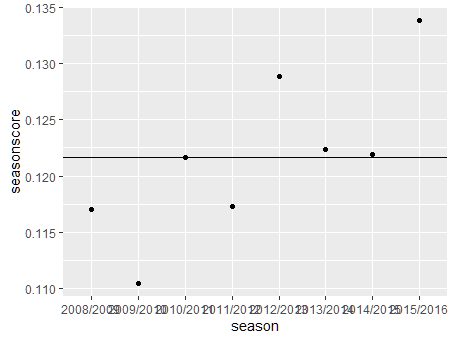
\includegraphics{season.png}
    \caption{seasonscore}
    \label{fig:season}
\end{figure}
An interesting condition was the season, with the proportion of underdog wins increasing over the years.

\begin{figure}[!ht]
    \centering
    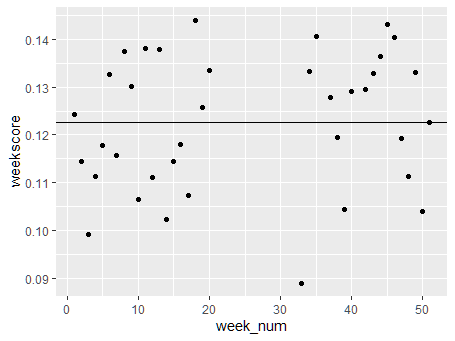
\includegraphics{week.png}
    \caption{weekscore}
    \label{fig:week}
\end{figure}
We notice an unusually high proportion of underdog wins from mid-August(wk33) to mid-November(wk46) which is during the first half of the season, and also early-May(wk19) at the very end of the season. A possible reason could be underdogs being more aggressive in the first half of the season when the league table is not set in stone and the favourites playing less hard at the very end of the season when their table positions may not be affected by losses. Next we look at perhaps the most directly correlated variable with underdog wins, the team attributes.

\section{Patterns in Team Attributes of Profitable Underdogs}
We seek to understand the key patterns of the winning underdogs through data analysis and visualisation. 
\subsection{Missing Data}
We start by looking at the team\_attributes.csv dataset.

$66.4\%$ of data of the attribute ``buildUpPlayDribbling" are missing, and their corresponding values of attribute ``buildUpPlayDribblingClass" were all set to ``Little". Considering such a high level of information loss, we drop these two columns in our analysis.

\subsection{Exploratory Data Analysis of Team Attributes}
In an attempt to have a thorough understanding of the dataset, some analysis leads us to the following discoveries:
\begin{itemize}
    \item Each numerical attribute takes integer value in the range $[20,80]$, following a roughly normal distribution. (See Figure \ref{fig:normal} for the QQ-plots)
    \begin{figure}[!ht]
        \centering
        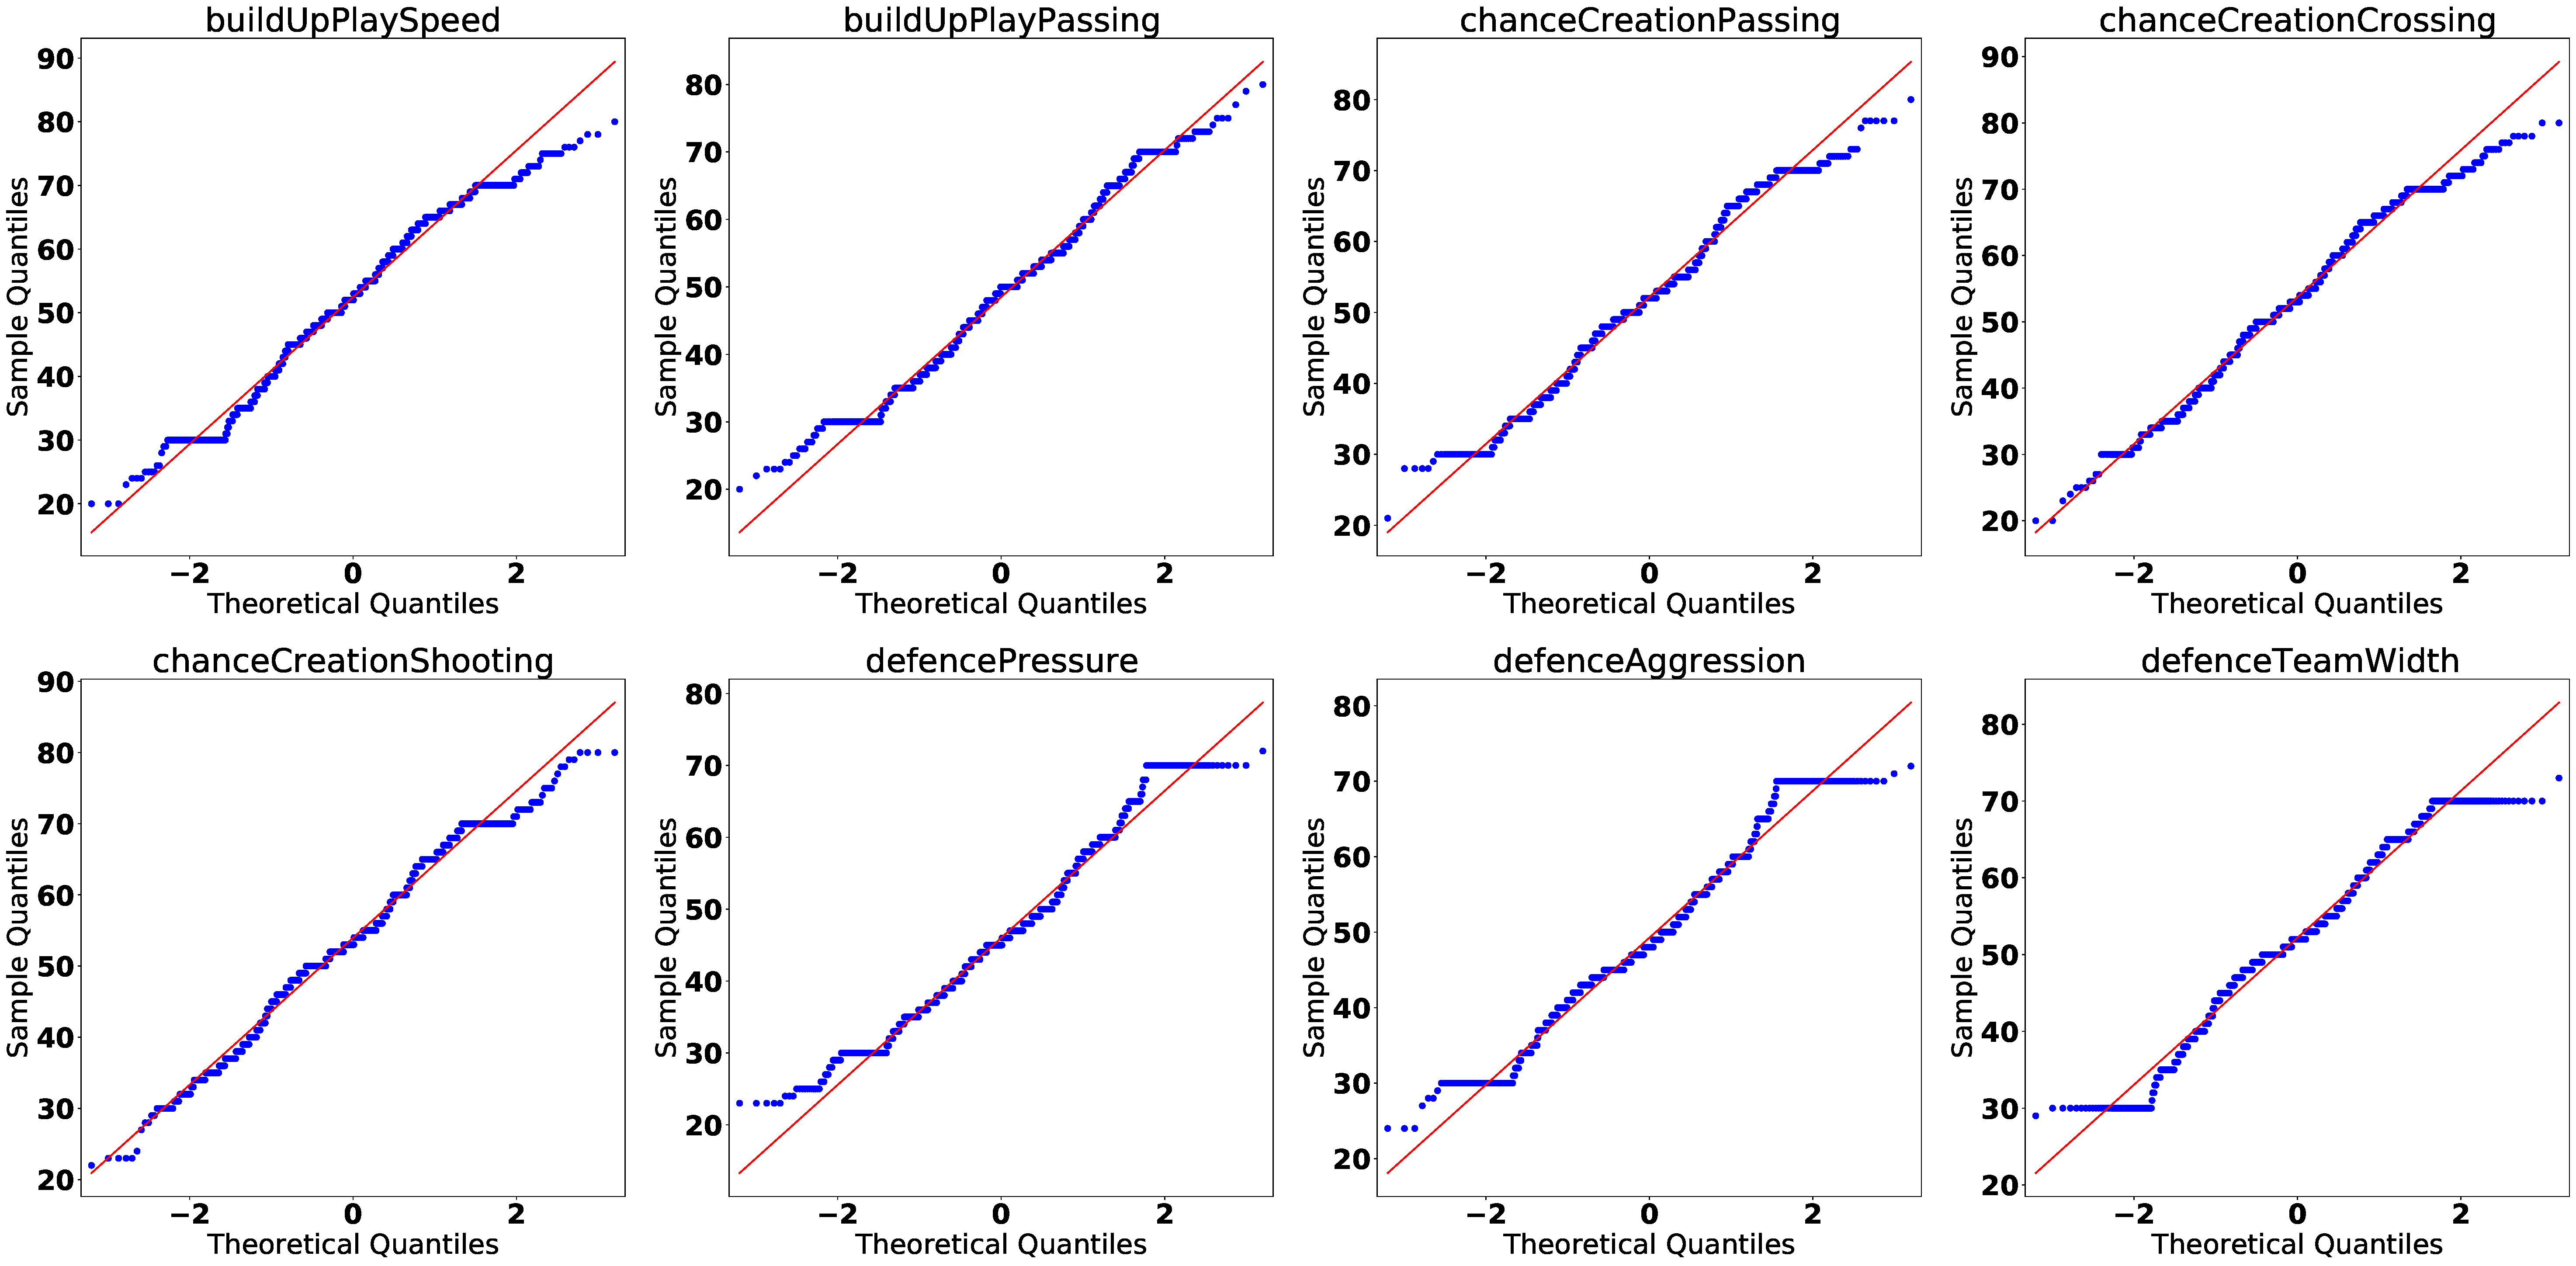
\includegraphics[width=15cm]{normal.pdf}
        \caption{QQ plot of numerical attributes}
        \label{fig:normal}
    \end{figure}
    
    \item Some of the categorical attributes are simply processed from the corresponding numerical attributes, and hence do not contain any additional information: e.g. ``buildUpPlayDribblingClass" classed the value of ``buildUpPlayDribbling" to be ``Slow" if the value is in the range $[20,33]$, ``Balanced" if the value is in the range $[34, 66]$,  ``Fast" if the value is in the range $[67,80]$. Other columns use the same classification threshold.
    \item Figure \ref{fig:corr} shows the correlation between the numerical attributes. We can see that there are relatively strong positive correlation between ``buildUpPlaySpeed'' and ``buildUpPlayPassing'', and among ``defencePressure'', ``defence Aggression'', ``defenceTeamWidth''.
    \begin{figure}[!ht]
        \centering
        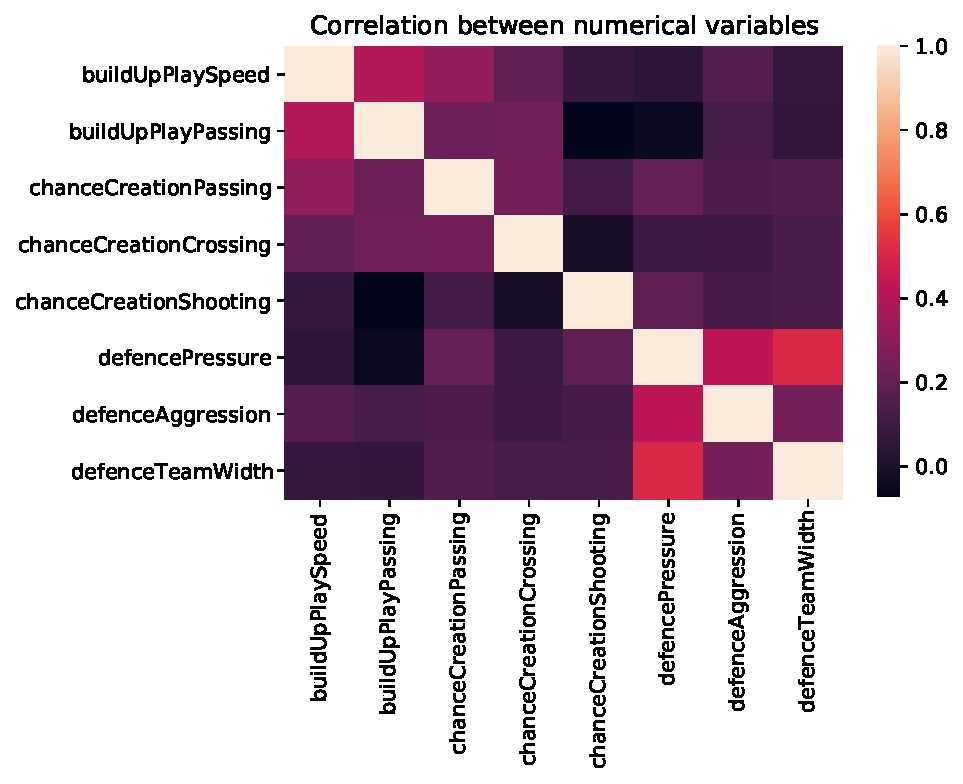
\includegraphics[width=10cm]{corr.pdf}
        \caption{Correlation between team attributes}
        \label{fig:corr}
    \end{figure}
    
    \item The dataset gives each team's attributes over several dates. Does each team tend to have roughly unchanged ratings over the years? We calculated the mean variance of each numerical attribute grouped by team, as given in \ref{tab:meanvar} As we can see the variance is quite large. Hence in the later analysis, we treated each team in different years essentially as different teams. i.e. we redefine the original team\_id as team\_id + year, for the sake of more accurate future analysis. 
    
    \begin{table}[!ht]
        \centering
        \begin{tabular}{ |c|c| } 
        \hline
        Attribute & Mean Variance \\
        \hline
        buildUpPlaySpeed   &       98.804197\\
        buildUpPlayPassing      &  84.513564\\
        chanceCreationPassing    & 79.838564\\
        chanceCreationCrossing   & 86.146776\\
        chanceCreationShooting  &  84.831204\\
        defencePressure         &  74.210219\\
        defenceAggression       &  77.362835\\
        defenceTeamWidth        &  67.778224\\
        \hline
        \end{tabular}
        \label{tab:meanvar}
        \caption{Variance of numerical attributes of         each team over time, taken the average }
    \end{table}
\end{itemize}

\subsection{Profitable Underdogs and Patterns In Their Attributes}
From Section 3.3, we identified the underdogs with a dogscore measuring profitability. We then explore the attributes of the profitable underdogs:

We define a three-dimensional rating for the teams, namely ``build up play score", ``chance creation score", ``defence" score. We can then identify the profitable underdogs among all underdogs' profiles, as shown in Figure \ref{fig:underdog3d}.

\begin{figure}[!ht]
    \centering
    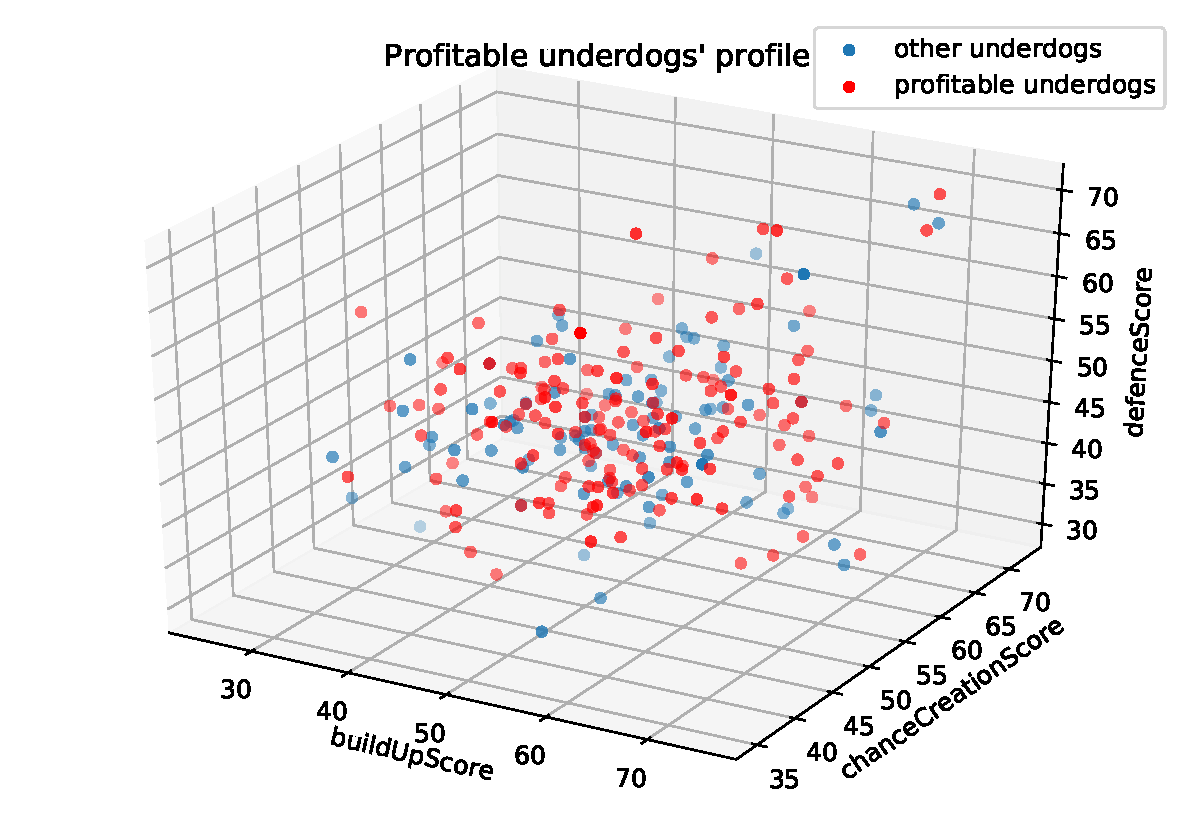
\includegraphics[width=10cm]{dog1.pdf}
    \caption{3D profile of the profitable underdogs among other underdogs}
    \label{fig:underdog3d}
\end{figure}

Also, we compare the numerical attributes of the profitable underdogs against all of the underdogs, the results are shown in Figure \ref{fig:underdog_attributes}. We can see that profitable underdogs are likely to have lower ``buildup play speed", higher ``chance creation crossing" and ``defence pressure".

\begin{figure}[!ht]
    \centering
    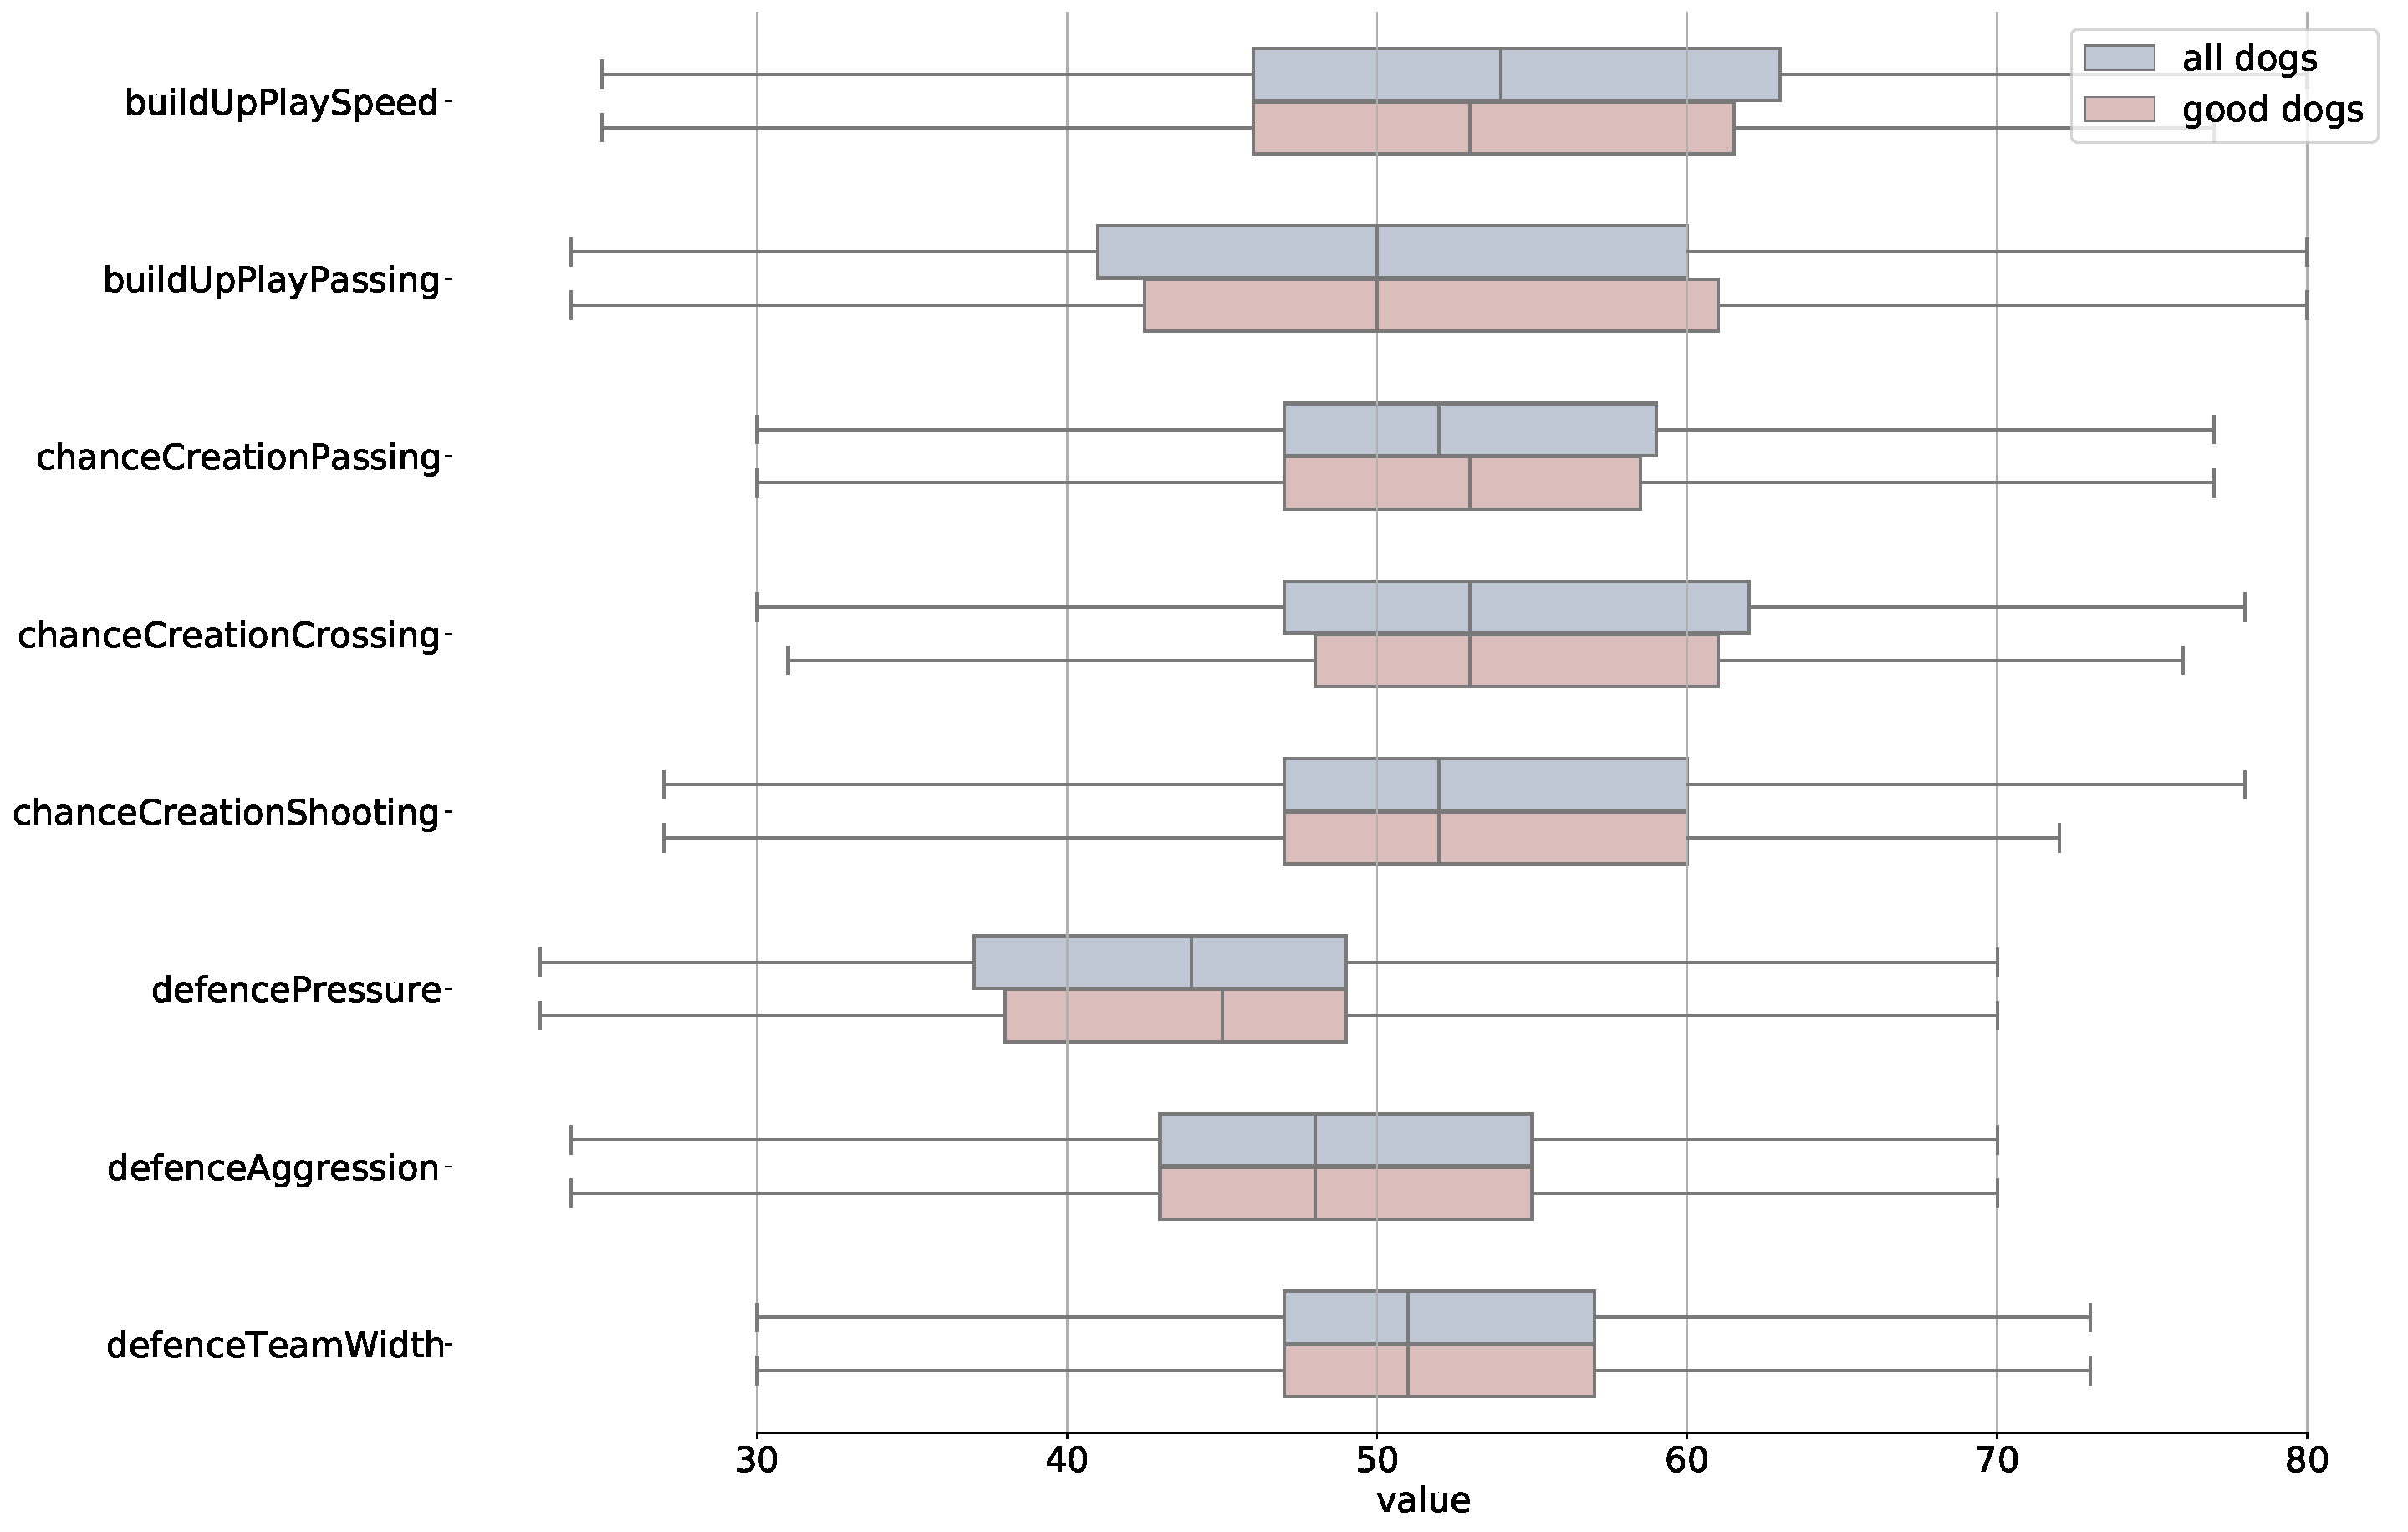
\includegraphics[width=15cm]{dog2.pdf}
    \caption{Profitable underdogs' numerical attributes}
    \label{fig:underdog_attributes}
\end{figure}

\subsection {Linear regression}
We fit a linear regression model $Y = X\beta + \epsilon$ for $Y = \text{dogscore}$, $X = \text{the vector of all team attributes}$. Preproceessing is done by normalising the numerical attributes. The correlation coefficients with respect to
each team attribute respectively is shown in the table below.
\begin{table}[!ht]
    \centering
    \begin{tabular}{|c|c|}
    \hline Team Attribute & correlation coefficient \\
    \hline buildUpPlayPassing & -0.10657641\\
    \hline chanceCreationPassing & 0.06743499 \\
    \hline chanceCreationCrossing & 0.01475563 \\
    \hline chanceCreationShooting' &  -0.08094743 \\
    \hline defencePressure & 0.00932558 \\
    \hline defenceAggression &  -0.2174565\\
    \hline defenceTeamWidth & 0.03256529\\
    \hline buildUpPlayPositioningClass & 0.15186524\\
    \hline chanceCreationPositioningClass & -0.07967342\\
    \hline defenceDefenderLineClass & 0.135266\\
    \hline
    \end{tabular}
    \caption{correlation coefficients of dogscore with respect to respective team attribute}
    \label{tab:my_label}
\end{table}

        

\section{Conclusion}

In conclusion, we explored the possibility of selective underdog betting, and by analysing match conditions and team attributes, we illuminate factors that lead to underdogs' surprise wins. Our findings may be fed to selected models in future to create a barometer to advise on specific underdog bets.






\end{document}